\documentclass[12pt,a4paper]{report}
\usepackage[utf8x]{inputenc}
\usepackage{ucs}
\usepackage{amsmath}
\usepackage{amsfonts}
\usepackage{amssymb}
\author{Michael Haas <haas@cl.uni-heidelberg.de>}
\title{Report Advanced Programming: Web-Scale Indexing for Information Retrieval}
\begin{document}
\maketitle
\section{Problem Description}
\label{ProblemDescription} 
For my final project, I chose to work on web-scale crawling and indexing. This is different from the original
project proposal which was mainly concerned with index generation on a fixed set of documents, e.g. those
found in an office setting. This index generation task is well suited for Hadoop, as the data is easily divided
into independent chunks for the Hadoop framework. It is typically sufficient to assign one or multiple files
to a mapper task, which yields the terms found in the document as intermediate keys and the document identifiers
as file names. The Hadoop framework then sorts the intermediate data so that each reducer gets a term with a list
of documents in which this term can be found. The process becomes somewhat more complicated if we move beyond toy examples
and compute relative term frequencies, but the data is still easily divided and it is straightforward how we can leverage
the sorting abilities of the framework to lessen the burden on the programmer.

In contrast, the web indexing task operates on an unknown set of documents which are discovered at run-time.
We parse and index hyperlink documents, which link to other hypertext documents. By following these links, we can
gradually discover the whole graph and expand our index. Additionally, a good web indexer is polite - it never overloads
the machines serving the documents and uses grace periods between indexing runs. Thus, we have two fundamental problems.
For one, we need to make the Hadoop framework aware of newly discovered documents so it can start jobs indexing them, which
in turn can lead to more newly discovered documents. As a consequence of constantly discovering new documents,
we need to remember which documents we have seen already and keep track of crawl dates to schedule re-crawls.
Second, we need to somehow avoid having multiple crawlers fetching
pages from the same server, thus increasing load impolitetely. These two problems effectively mean
we have data dependencies between
individual indexing runs (or rather documents) which do not exist in the simple document indexing task. We would need the Hadoop
tasks to talk to each other to avoid trouble which is against the functional nature of the Hadoop Map-Reduce approach. It
also is a performance nightmare.
\section{My Approach}
I choose to implement three Map-Reduce jobs in an iterative pipeline: the Indexer, the IndexMerger and the WebDBMerger. The Indexer
deals with document retrieval via HTTP and generation of intermediate index files while the WebDBMerger
manages the constraints we identified in the \ref{ProblemDescription}. The WebDBMerger merges the newly discovered URLs
with the WebDB, the database of already known URLs. URLs are grouped by domain. The WebDB serves as the input for the
Indexer job. It is guaranteed that all URLs for a given domain are handled by one single reducer, which avoids the need
for synchronisation across reducers and allows easy implementation of politeness measures.
The IndexMerger merges multiple index files, e.g. the result
of multiple reduce tasks in the Indexer, into a single file and sorts the data for faster retrieval.
The pipeline is used in iterations: after each run, the pipeline is restarted and operates on the output of the previous run. Please
see \ref{FlowChart} for an overview of the system.
\begin{figure}
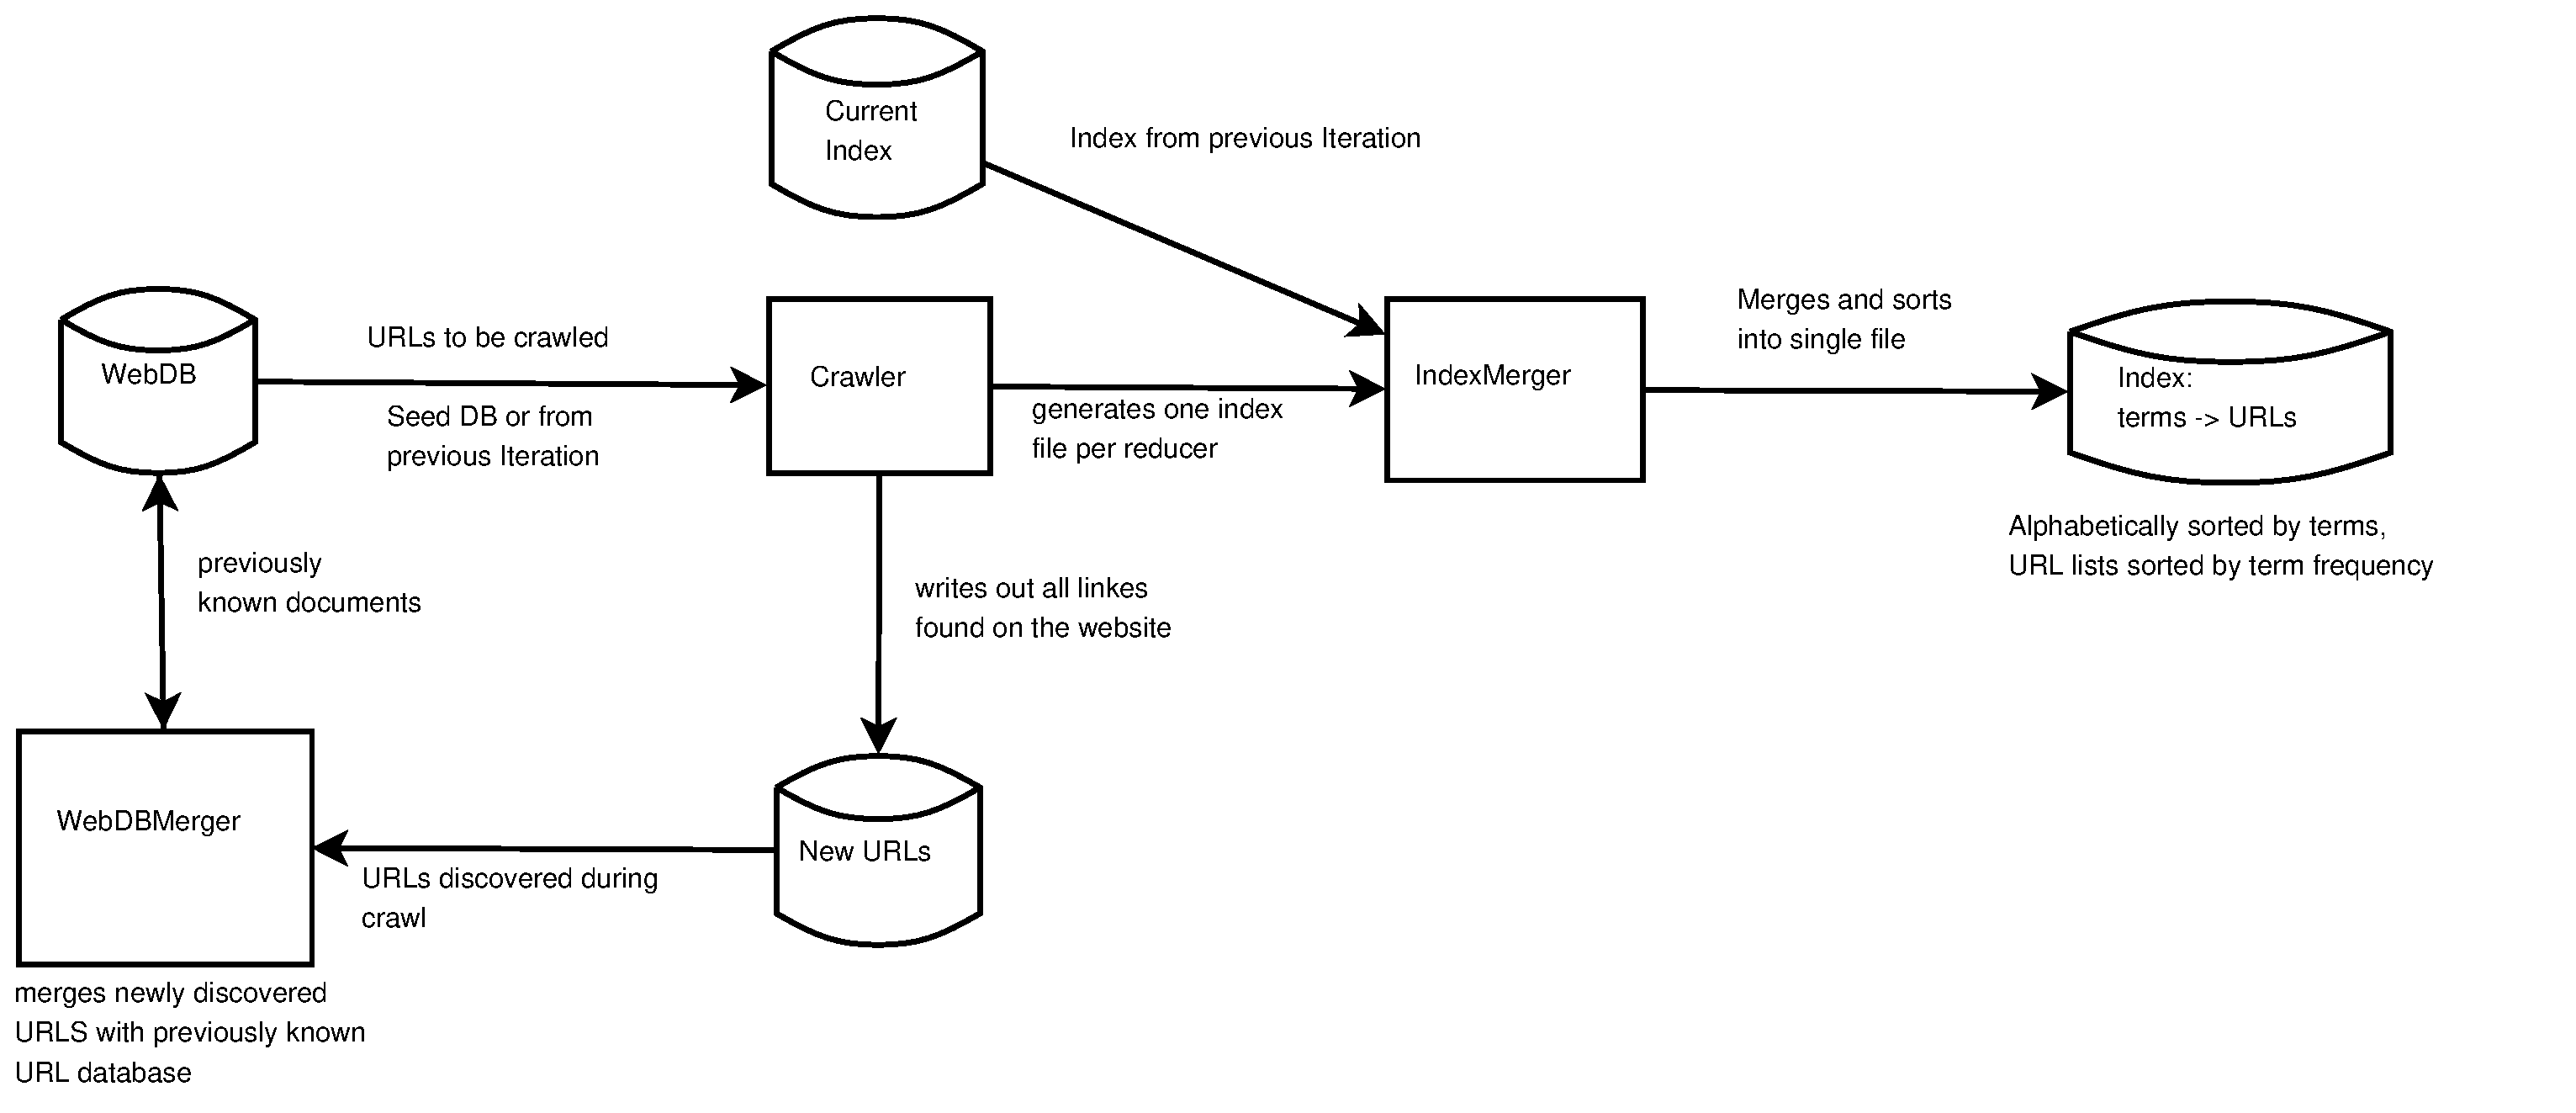
\includegraphics[scale=1]{Diagramm1.eps} 
\caption{Flow chart of the system}
\label{FlowChart} 
\end{figure}

\subsection{The Indexer}
The input of the Indexer is the WebDB. The WebDB is a mapping from host names to lists of tuples of URLs and time stamps pointing to last retrieval date. The output of the Indexer is a mapping from terms to lists of tuples of URLs and term frequency. On the side, the Indexer writes out any newly discovered URLs into a separate file. All input and output
files are instances of SequenceFile.
The mapper receives the domain name of the WebDB entry as key and the list of URLs and time stamps as value. For each URL, it checks the time stamp of the last crawl
to decide if a re-crawl is warranted.\footnote{In a real-world application, we would look at the sitemap do determine individual re-crawl frequencies}. If the time stamp is older
than 5 minutes, the mapper fetches the URL, checks the content-type header for HTML content\footnote{The HTML parser will happily accept binary PDF files, putting binary noise into the index} and processes the HTML using the Jericho HTML parser\footnote{http://jericho.htmlparser.net/docs/index.html}. The resulting parse tree of the document is traversed for
outgoing links to other documents which are written into the "fresh-urls" directory. The full text of the document is extracted from the parse tree, split into terms with a
simple tokenizer and sent to the reducer with the term as key and the posting (URL and frequency) as value. The reducer collects all postings for a term and serializes it into a sequence file. Having multiple reducers speeds up the process considerably. Note that the Indexer itself does not update the WebDB with the newly discovered URLs, this is the job
of the WebDBMerger. We do not feed the new URLs back directly into the Indexer process, thus avoid the need for expensive task synchronization.
\subsection{The WebDBMerger}
The input of the WebDBMerger consists of two directories. One directory holds a SequenceFile with the old WebDB, the second directory is the "fresh-urls" directory holding the newly
discovered URLs. Both have the same format: a mapping from Domain to a list of tuples of URLs and timestamps contained in a SequenceFile. For the newly discovered URLs,
the timestamp will indicate we have not seen them yet.
As a result of this simple design, the Mapper simply is the identity function. The Hadoop framework proceeds then groups the URLs by the key, i.e. the domain and hands them
to the Reducer. Here, we eliminate duplicate URLs, preferring the fresher timestamp to prevent premature re-crawls. The output of the Reducer is the new WebDB which
serves as input for the Indexer.
Duplicate URLs with different timestamps happen for a few reasons:
\begin{itemize}
\item Two sites pointing to the same new document
\item A site points to a document already in the WebDB
\item The Indexer wrote its currently crawled URL with the new timestamp to fresh-urls
\end{itemize}
This way, the WebDBMerger also serves as an update mechanism for the time stamp of the currently crawled URL. Once the crawl is done,
the Indexer considers the currently crawled URL as a new URL and writes it to the "fresh-urls" directory with the current timestamp.
The WebDBMerger will then see both the new entry and the old entry in the WebDB and throw away the old entry when merging. Updating the
previously known URLs with new timestamps in a process separate from the Indexer is another way I avoid synchronisation between Indexer tasks.
Running the WebDBMerger with multiple Reducer tasks has a nice side effect of producing multiple output files, each holding a part
of the WebDB. By default, the Hadoop framework will start multiple map tasks for each input file in subsequent iterations,
speeding up the crawl process considerably.
\subsection{The IndexMerger}
The IndexMerger merges the old index from previous iterations with the (possibly many)\footnote{Number of output files depends on number of Reduce tasks in the Indexer} output files of the Indexer process. While merging the files, the output is sorted by term (done by the framework) and the URLs are sorted by term frequency. This job
uses the value-to-key conversion pattern to offload the sorting by term frequency to the Hadoop framework.
The input for the IndexMerger consists of the old index file and the output files of the Indexer process. Both are SequenceFiles holding mappings from terms to posting lists (URL and term frequency). The Mapper yields TermCount instances representing tuples (term,frequency) as key and an URL as value with a custom partitioner shuffling keys with the same term to the same Reducer. The TermCount class features a custom implementation of the WritableComparable interface to guarantee that keys are first sorted by term, then by frequency\footnote{It has since come to my attention that it is not particularly useful to sort the posting lists by frequency. It is much more useful to sort by URL to allow fast lookup in O(log(N)). The same process as described here would work for this: simply use the URL instead of the frequency in the composite intermediate key}.
\subsection{Retrieval}
Retrieval is an afterthought in this project, as the main focus is on distributed crawling and indexing. A simple retrieval script
which runs on the local machine is provided. It uses a boolean retrieval model and can handle multiple search terms
which are either linked with AND or with OR.
\section{Results}
The test run for the system starts with a seed file consisting of three documents:
\begin{itemize}
\item  http://www.cl.uni-heidelberg.de
\item http://de.wikipedia.org/wiki/Wikipedia:Hauptseite
\item http://www.uni-heidelberg.de
\end{itemize}
Each crawled website can contribute up to 50 new URLs to the WebDB\footnote{This restriction prevents early size explosion of the WebDB}.

\begin{table}
\label{ResultTable} 
\begin{tabbing}
Iteration \= Size WebDB \= Fresh URLs \= Time elapsed \\
1 \> 3  \> 126 \> 53s\\ 
2 \> 100 \> 3701 \> 266s\\
3 \> 2260 \> 85914 \> 5694s\\

\end{tabbing}
\caption{Results with three input documents. Total time: 6075s}
\end{table}

We can see that the size of the WebDB grows exponentially. Starting from three seed documents, we find 126 fresh URLs of which 100 are unique after the WebDBMerger run.
For these 100 URLs, we find 3701 fresh URLs, which leads to 85914 fresh URLs in the third iteration. Given that every document may only contribute 50 fresh URLs
to the WebDB, the WebDB grows at $O(50^n)$, with $n$ being the iteration. This growth will, of course, slow down as we find more and more documents we already know.

\section{Running the code yourself}
The code is either obtained via tarball or from \url{https://github.com/mhaas/distributed-crawl}. The code is built using Apache Maven, which will download
all dependencies and compile the source code. To obtain an easily deployable jar file containing all dependencies, run \texttt{mvn install hadoop:pack} inside the source directory.
The distribution contains several Bash scripts. To generate an initial WebDB from a seed file \texttt{seed.txt}, simply run \texttt{./text2webdb.sh seed.text} and move the resulting \texttt{webdb.dat} into the right directory: \texttt{rm -rf webdb \&\& mkdir webdb \&\& mv webdb.dat webdb/}.
To start the crawl process, execute \texttt{run.sh} with the number of iterations as first argument: \texttt{./run.sh 2}. The script will upload the webdb,
clean up the HDFS and start the whole pipeline\footnote{uses de.hd.cl.haas.distributedcrawl.App}. After the specified number of iterations, \texttt{run.sh} will copy
the index file and any intermediate directories to disk for further inspection.
\subsection{Document retrieval}
Given the index, the \texttt{query.sh} wrapper script\footnote{uses de.hd.cl.haas.distributedcrawl.search.Searcher} allows document retrieval from the index.
\begin{verbatim}
$ ./query.sh index-raw/part-r-00000 AND Computerlinguisten
Got result: http://www.cl.uni-heidelberg.de/interest/index.mhtml
$ ./query.sh index-raw/part-r-00000 OR Computerlinguisten Computerlinguistik
Got result: http://de.wikipedia.org/wiki/Portal:Geist_und_Gehirn
Got result: http://www.cl.uni-heidelberg.de/interest/index.mhtml
\end{verbatim}
The first parameter specifies the index file, the second parameter specifies whether to link search terms with AND or OR. Finding the correct index file is somewhat tricky as
the purpose of a directory changes depending on the iteration count as input directories become output directories for the IndexMerger. For uneven iteration counts, the index can be found in \texttt{index-raw}, for even iteration counts in \texttt{index-sorted}. Generally speaking, the directory with only one part\_* file will be have the correct index file.\footnote{It is not possible to rename directories in HDFS, so I choose to change the directory purpose instead of copying the files around}.
\subsection{Writing your own seed file}
If you would like to extend the \texttt{seed.txt} file or write your own file, the format is quite simple.
Each line holds the list of URLs for a given host. The host name is the first entry of the line, the rest of the entries
on that line are considered URLs which are indexed. Entries on a given line are delimited by TAB. Note that the file does not have a terminal newline.
\begin{verbatim}
foo.bar.baz\\thttp://foo.bar.baz/index.html\\thttp://foo.bar.baz/cats.html\n
fuu.bar.baz\\thttp://fuu.bar.baz/main.php\\thttp://fuu.bar.baz/cakes.php
\end{verbatim}

\section{Closing thoughts}
Many things could not be implemented, as web-scale indexing is a project bigger than what anyone could do in a few weeks. Support for additional document types
such as PDF comes to mind, as well as proper support for robots.txt exclusion files whose direction are respected by well-behaved web crawlers. Using hashes of URLs instead of Strings in the Index file could speed up retrieval considerably while also saving space in the index. However,
these items do not directly relate to the core problem of leveraging the Hadoop framework to build web-scale crawling and indexing, so I will focus on those.
\\
As for efficient retrieval, having the ability to perform fast searches would be beneficial. This can be achieved using the MapFile class which maintains an index on
key positions in a SequenceFile. A fast binary search in O(log(n)) would be possible using the MapFile, but there is no MapFileOutputFormat in Hadoop 0.20.2 which can be used with the Reducer in the IndexMerger\footnote{There is a deprecated version of the class available which can't be used as drop-in replacement}. This has been rectified in newer Hadoop releases.
\\
In table \ref{ResultTable}, we can see that the duration of the pipeline runs and the size of the WebDB increases exponentially. This causes unacceptable delays in updating the index to the point where we have to crawl the entire web graph before we can update the index. To lessen this delay, it might be possible to run the IndexMerger concurrently. The IndexMerger does not depend on all input data to be processed successfully, but it remains to be seen if the output of
the reducer of the Indexer is usable before the job is actually finished. However, HDFS semantics would definitely allow a model where the IndexMerger already reads from files while
the Indexer is still running. As an alternative, it is possible to start the Indexer again with a separate output directory while the IndexMerger is still running.
\\
Another approach to reduce turnover time would be the segmentation of the WebDB into several segments. This could simply be done on alphabetical order, e.g.
crawl domains whose initial letter are in A-D, then E-H, and run the IndexMerger after each crawl.
A more interesting alternative would be the segmentation according to crawl frequency: frequently updated documents go into their own segment, while rarely updated documents go into their own segment and are crawled less frequently.
\\
Each Mapper task in the Indexer spends quite some time waiting for network I/O. By using the MultithreadedMapper, we could use each Mapper instance much more effectively by allowing more throughput.
\\
Good values for the number of reduce task still have to be found. I noticed that raising the number of reducers for the WebDBMerger does not only speed up the WebDBMerger itself,
but also the Indexer process as the increased number of input files allows more mapper tasks to be run in parallel. The number of mapper tasks should be increasable without increasing the number of input files, but it is not entirely clear to me how the generation of the input split for single files can be controlled. In any case, raising the number of reducers from the default of 1 can help performance, but it can also cause unnecessary I/O across the cluster which slows down the computation, especially if it's just done for the side effect of increasing the number of mapper tasks for the Indexer.
\\
Combiners could help speed up the jobs considerably. Especially for the WebDBMerger and the IndexMerger, where many intermediate key-value pairs are generated, the in-mapper combiner could reduce I/O load and sorting cost.






\end{document}